\documentclass{article}
\usepackage[utf8]{inputenc}

\usepackage{tikz}
\usetikzlibrary{positioning}
\usetikzlibrary{calc}

\begin{document}

%------------------------------------------------------------------------------
\newcommand{\yslant}{-0.3}
\newcommand{\xslant}{0}
%Introductory example
\begin{figure}[p]
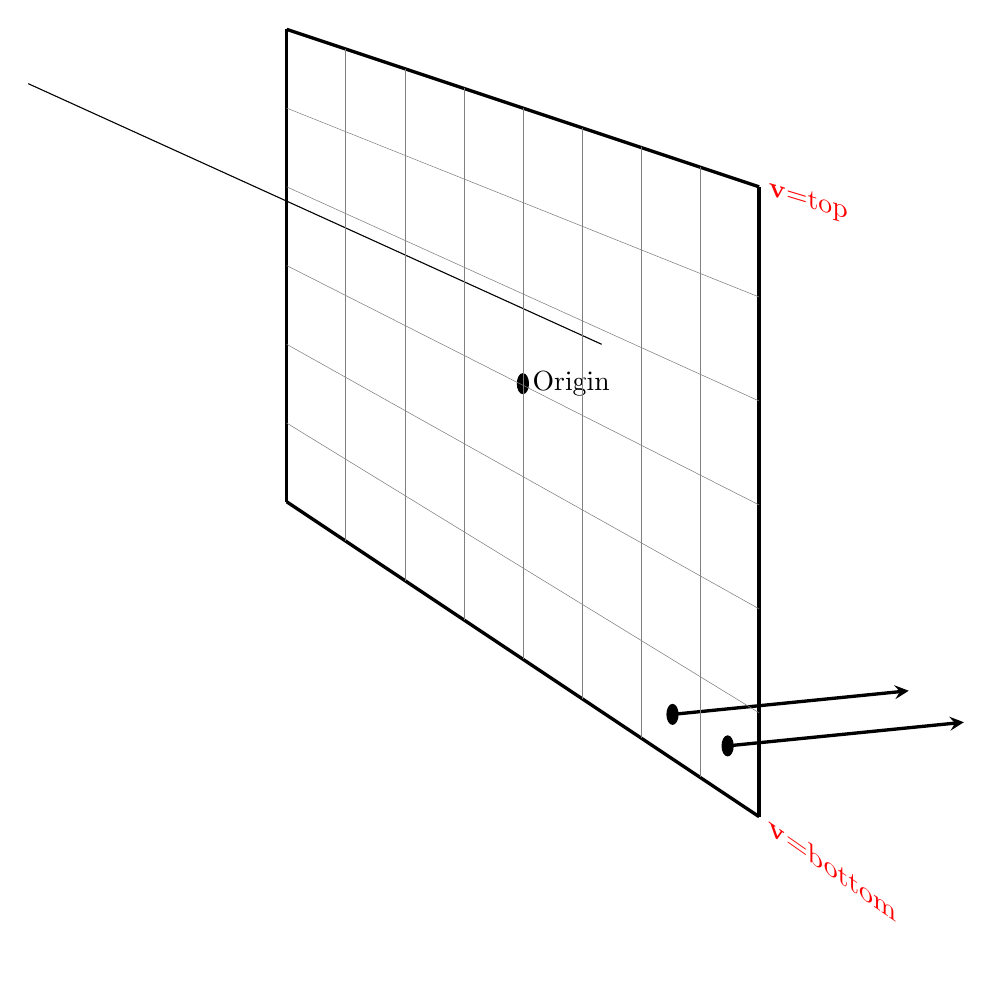
\begin{tikzpicture}[scale=2,every node/.style={minimum size=1cm},on grid, >=stealth]
    \tikzstyle help lines=[color=gray,very thin]
    \tikzstyle border lines=[color=black,very thick]

\begin{scope}[
		%yshift=-120,
		%every node/.append style={yslant=\yslant,xslant=\xslant},
		%yslant=\yslant,xslant=\xslant
	] 
		 % Labels:
		\fill[red]
			(2,1) node[yslant=-0.3, right, scale=1] {$\mathbf{v}$=top}
			(2,-3) node[yslant=-0.7, right, scale=1] {$\mathbf{v}$=bottom}	;
;
\end{scope}

\coordinate (vanishingpoint) at (-10,5);
\draw (1,0) -- ($(1,0)!4cm!(vanishingpoint)$);

    % (i=4, j=3)
    \filldraw[black] (-1+4*0.375, -1 + 3*0.25) ellipse (1.0pt and 1.8pt) node[anchor=west] {Origin};
    \filldraw[yshift=-2.3cm, ->, xshift=1.3cm,black] (-1+4*0.375, -1 + 3*0.25) ellipse (1.0pt and 1.8pt);
    \draw[yshift=-2.3cm, ->, xshift=1.3cm, very thick] (-1+4*0.375, -1 + 3*0.25) -- (2,-0.1); % X axis
    \filldraw[yshift=-2.1cm, ->, xshift=0.95cm,black] (-1+4*0.375, -1 + 3*0.25) ellipse (1.0pt and 1.8pt);
    \draw[yshift=-2.1cm, ->, xshift=0.95cm, very thick] (-1+4*0.375, -1 + 3*0.25) -- (2,-0.1); % X axis
%\draw[gray, thick] (-1,2) -- (2,-4); % longer diagonal
%\draw[gray, thick] (-1,-1) -- (2,1); % shorter diagonal

    \draw[style=border lines] (-1, 2) -- (-1,-1); % left border
    \draw[style=border lines] ( 2, 1) -- ( 2,-3); % right border
    \draw[style=border lines] (-1, 2) -- ( 2, 1); % top border
    \draw[style=border lines] (-1,-1) -- ( 2,-3); % bottom border
    
    % Vertical Y range on right: [-3, 1], increment: 0.66
    % vertical Y range on left: [-1,2]: increment 0.5
    \foreach \i in {1,...,5}
        \draw[style=help lines] (-1,\i*0.5-1) -- (2,\i*0.66 - 3);
    % Horizontal X range on top: [-1, 2], increment is 3/8 = 0.375
    % The increment formula is -1 + \i*0.375 for both Xs.
    % Horizontal X range on bottom: [-1,2]: increment is 3/8 = 0.375
    % Y increment at the top begins at Y=2 (left), and goes to Y=1 (right), so the increment is 1/8=0.125
    % The increment formula is 2 - \i*0.16
    % Y increment at the bottom begins at Y=-1 (left), and goes to Y=-3 (right), so the increment is 2/8=0.25
    % The increment formula is -1 - \i*0.33
    \foreach \i in {1,...,7}
        \draw[style=help lines] (-1+\i*0.375, 2-\i*0.125) -- (-1+\i*0.375, -1 - \i*0.25);
    %2-\i*0.16
\end{tikzpicture}
\end{figure}
%------------------------------------------------------------------------------


%------------------------------------------------------------------------------
%Introductory example
\begin{figure}[p]
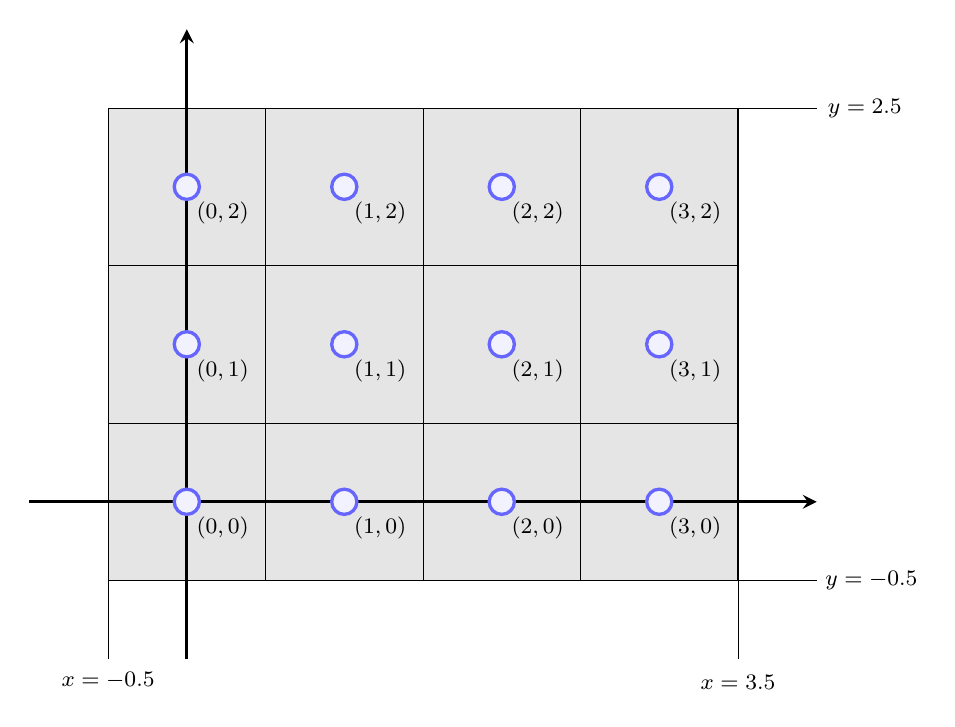
\begin{tikzpicture}[>=stealth, scale=2]
  % definition of a basic style.
  \tikzstyle help lines=[color=black,very thin]
  % The background rectangle that works as a filling in rectangle
  \filldraw[fill=gray!20!white, step=1,  xshift=-0.5cm, yshift=-0.5cm]
    (0cm,0cm) rectangle (4cm,3cm);
  % The grid
  \draw[step=1, style=help lines, xshift=-0.5cm, yshift=-0.5cm]
    (0cm,0cm) grid (4cm,3cm);

  % The coordinate axes.
  \draw[->, very thick] (-1.,0) -- (4,0); % X axis
  \draw[->, very thick] (0,-1.) -- (0,3); % Y axis
  
  % support vertical, horizontal lines.
  \draw[very thin] (3.5,2.5) -- (4,2.5) node[xshift=1.2cm,anchor=east] {\footnotesize$y=2.5$};
  \draw[very thin] (3.5,-0.5) node{} -- (4,-0.5) node[xshift=1.4cm,anchor=east] {\footnotesize$y=-0.5$};
  \draw[very thin] (3.5,-0.5) -- (3.5,-1.) node[yshift=-0.5cm,anchor=south] {\footnotesize$x=3.5$};
  \draw[very thin] (-0.5,-0.5) -- (-0.5,-1.) node[yshift=-0.5cm,anchor=south] {\footnotesize$x=-0.5$};

  % Row of circles
  \foreach \x in {0,...,3}
        \filldraw [color=blue!60, fill=blue!5, very thick] (\x,0) circle (0.08cm);
  \foreach \x in {0,...,3}
        \filldraw [color=blue!60, fill=blue!5, very thick] (\x,1) circle (0.08cm);
  \foreach \x in {0,...,3}
        \filldraw [color=blue!60, fill=blue!5, very thick] (\x,2) circle (0.08cm);
  % Coordinates
  \foreach \x in {0,...,3}
    \draw (\x cm,-0.3cm) node[anchor=south west] {\footnotesize$(\x, 0)$};
  \foreach \x in {0,...,3}
    \draw (\x cm,0.7cm) node[anchor=south west] {\footnotesize$(\x, 1)$};
  \foreach \x in {0,...,3}
    \draw (\x cm,1.7cm) node[anchor=south west] {\footnotesize$(\x, 2)$};
    
  %  \filldraw[color=red!60, fill=red!5, very thick](-1,0) circle (1.5);
\end{tikzpicture}
\end{figure}
%------------------------------------------------------------------------------
    
%------------------------------------------------------------------------------
%Points, lineas and curves
\begin{figure}[p]
\begin{tikzpicture}
\draw (-2,0) -- (2,0);
\filldraw [gray] (0,0) circle (2pt);
\draw (-2,-2) .. controls (0,0) .. (2,-2);
\draw (-2,2) .. controls (-1,0) and (1,0) .. (2,2);

\end{tikzpicture}
\end{figure}
%------------------------------------------------------------------------------


%------------------------------------------------------------------------------
%Circles and arcs
\begin{figure}[p]
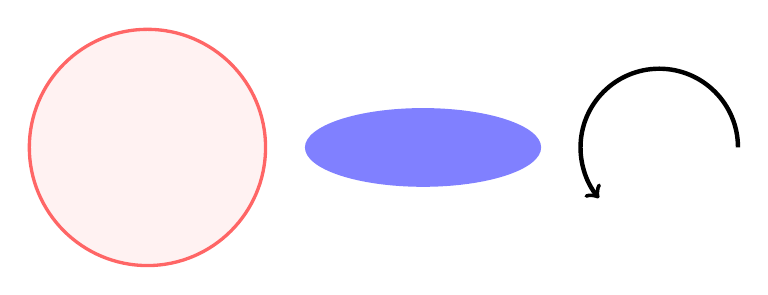
\begin{tikzpicture}
\filldraw[color=red!60, fill=red!5, very thick](-1,0) circle (1.5);
\fill[blue!50] (2.5,0) ellipse (1.5 and 0.5);
\draw[ultra thick, ->] (6.5,0) arc (0:220:1);
\end{tikzpicture}
\end{figure}
%------------------------------------------------------------------------------



%------------------------------------------------------------------------------
%Polygons
\begin{figure}[p]
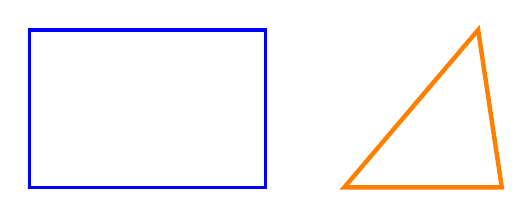
\begin{tikzpicture}
\draw[blue, very thick] (0,0) rectangle (3,2);
\draw[orange, ultra thick] (4,0) -- (6,0) -- (5.7,2) -- cycle;
\end{tikzpicture}
\end{figure}
%------------------------------------------------------------------------------


%------------------------------------------------------------------------------
%Diagram
\begin{figure}
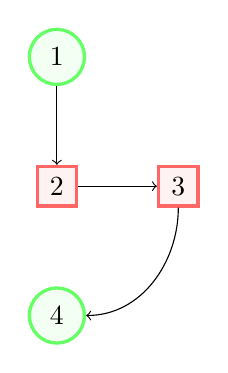
\begin{tikzpicture}[
roundnode/.style={circle, draw=green!60, fill=green!5, very thick, minimum size=7mm},
squarednode/.style={rectangle, draw=red!60, fill=red!5, very thick, minimum size=5mm},
]
%Nodes
\node[squarednode]      (maintopic)                              {2};
\node[roundnode]        (uppercircle)       [above=of maintopic] {1};
\node[squarednode]      (rightsquare)       [right=of maintopic] {3};
\node[roundnode]        (lowercircle)       [below=of maintopic] {4};

%Lines
\draw[->] (uppercircle.south) -- (maintopic.north);
\draw[->] (maintopic.east) -- (rightsquare.west);
\draw[->] (rightsquare.south) .. controls +(down:7mm) and +(right:7mm) .. (lowercircle.east);

\end{tikzpicture}
\end{figure}

%------------------------------------------------------------------------------


%------------------------------------------------------------------------------
%List of available colors 

\begin{figure}[p]

\begin{tikzpicture}
\filldraw[black] (0,0) rectangle (2,2);
\filldraw[red] (3,0) rectangle (5,2);
\filldraw[green] (6,0) rectangle (8,2);
\filldraw[blue] (9,0) rectangle (11,2);
\filldraw[cyan] (1,-1) rectangle (3,-3);
\filldraw[magenta] (4,-1) rectangle (6,-3);
\filldraw[yellow] (7,-1) rectangle (9,-3);
\end{tikzpicture}
\end{figure}
%------------------------------------------------------------------------------


%------------------------------------------------------------------------------
%Different levels of thickness
\begin{figure}[p]
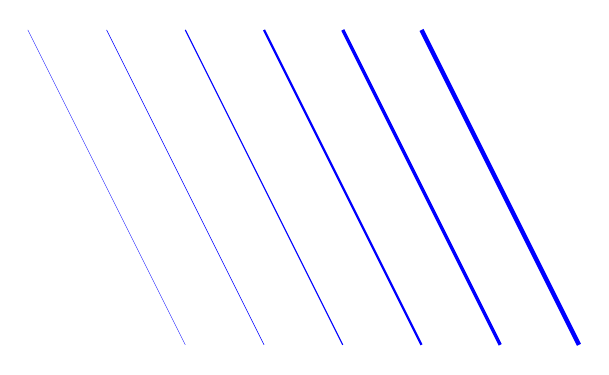
\begin{tikzpicture}
\draw[blue, ultra thin] (-1,2) -- (1,-2);
\draw[blue, very thin] (0,2) -- (2,-2);
\draw[blue, thin] (1,2) -- (3,-2);
\draw[blue, thick] (2,2) -- (4,-2);
\draw[blue, very thick] (3,2) -- (5,-2);
\draw[blue, ultra thick] (4,2) -- (6,-2);
\end{tikzpicture}
\end{figure}
%------------------------------------------------------------------------------

\end{document}

